\documentclass[11pt]{article}
\usepackage[utf8]{inputenc}
\usepackage[margin=1in]{geometry}
\usepackage{tabularx}
\usepackage{enumitem}
\usepackage{hyperref}
\usepackage{graphicx} % Required for inserting images
\usepackage{float}

\begin{document}

\begin{center}
    \huge \textbf{Meeting Minutes: Project Handoff} \\
    \large \textbf{Project:} Venue Booking Management System (VBMS) \\
    \large \textbf{Subject:} Code Review and Test Plan Foundation \\
    \rule{\textwidth}{0.4pt}
\end{center}

\section*{Meeting Information}
\begin{tabularx}{\textwidth}{l X}
    \textbf{Date:} & April 10, 2024 \\
    \textbf{Time:} & 16:47 -- 23:05 (Asynchronous Communication) \\
    \textbf{Location:} & Digital Coordination Channel (WhatsApp) \\
    \textbf{Participants:} & Abdul Wasay Imran (Testing Team), Maryam (Development Team) \\
\end{tabularx}

\section*{1. Objective}
The primary goal of this session was to acquire the source code, Software Requirement Specification (SRS), and system architecture details for the Venue Booking Management System to initiate Phase 2 of the Software Testing Project.

\section*{2. Functional Overview}
The system is built around three primary user roles:
\begin{itemize}[noitemsep]
    \item \textbf{Student:} Can browse buildings/rooms and book them. Includes logic for "Already Booked" status and "Time Conflict" validation.
    \item \textbf{Program Office (PO):} Responsible for the approval workflow (Accepting/Rejecting booking requests).
    \item \textbf{Admin:} Possesses full privileges, including request management and the ability to modify the infrastructure (Adding new buildings and rooms).
\end{itemize}

\section*{3. Technical Specifications \& Access}
\begin{itemize}
    \item \textbf{Repository:} \url{https://github.com/AmanTheDrummer/IBA-VBMS}
    \item \textbf{Active Branch:} \texttt{full-fix}
    \item \textbf{Environment Setup:} \texttt{npm run start:dev} (Backend) and \texttt{npm run dev} (Frontend).
\end{itemize}

\section*{4. Test Data Provided}
The following credentials were provided for the execution of functional test cases:
\begin{center}
\begin{tabular}{|l|l|l|}
\hline
\textbf{Role} & \textbf{Username/ERP} & \textbf{Password} \\ \hline
Admin & admin & admin123 \\ \hline
Program Office & po001 & password \\ \hline
Student & 12345 & password \\ \hline
\end{tabular}
\end{center}

\section*{5. Key Decisions}
\begin{itemize}[noitemsep]
    \item The SRS PDF will be used as the ground truth for Expected Results.
    \item Testing Team will analyze the API structure within the source code to develop unit test cases.
\end{itemize}



\section{Communication Transcript}
The following table logs the primary correspondence regarding the handoff of the system components.

\renewcommand{\arraystretch}{1.5}
\begin{tabularx}{\textwidth}{|l|l|X|}
\hline
\rowcolor{headergray} \textbf{Time} & \textbf{Sender} & \textbf{Message / Action} \\ \hline
16:47 & A. Wasay & Requested SRS, project idea, video demo, and API code access for unit testing. \\ \hline
17:06 & Maryam & Shared \texttt{srs.pdf} and confirmed access request. \\ \hline
22:15 & Maryam & Shared GitHub Repository link (\texttt{full-fix} branch). \\ \hline
22:16 & Maryam & Provided deployment commands: \texttt{npm run start:dev} and \texttt{npm run dev}. \\ \hline
22:17 & Maryam & Provided test credentials for Admin, PO, and Student roles. \\ \hline
23:05 & Maryam & Provided audio briefing explaining the role-based dashboard logic. \\ \hline
\end{tabularx}

\vfill
\begin{center}
    \small \textit{Minutes recorded by Abdul Wasay Imran}
\end{center}



\clearpage
\newgeometry{margin=0.5in}
\appendix

\section{Appendix: Communication Log}
The following screenshot documents...

\begin{figure}[H] % <--- CAPITAL H forces it to stay here
    \centering
    % Use height instead of width to make sure it fits vertically
    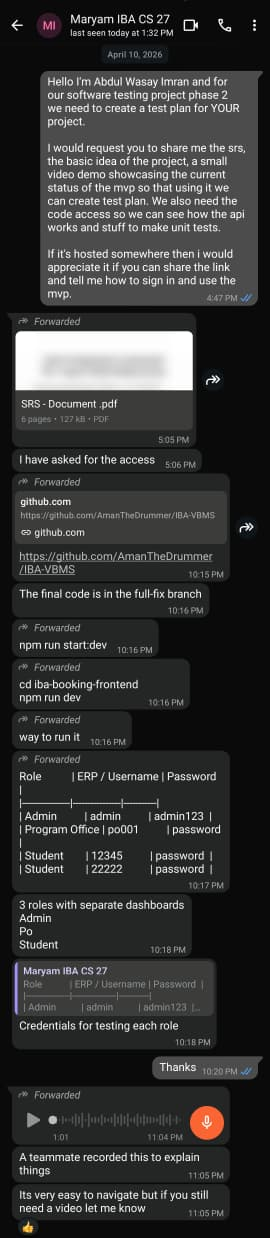
\includegraphics[height=0.85\textheight, width=\textwidth, keepaspectratio]{chat_log.jpeg} 
    \caption{WhatsApp communication with the development team (April 10, 2024)}
    \label{fig:chat_log}
\end{figure}

\end{document}